\chapter{Architektura projektu}
\section{Opis komponentów}
Rysunek \ref{fig:architecture} przedstawia ogólny zarys architektury projektu. Szczegółowe elementy zostały opisane poniżej.

\begin{figure}[htbp]
\centering
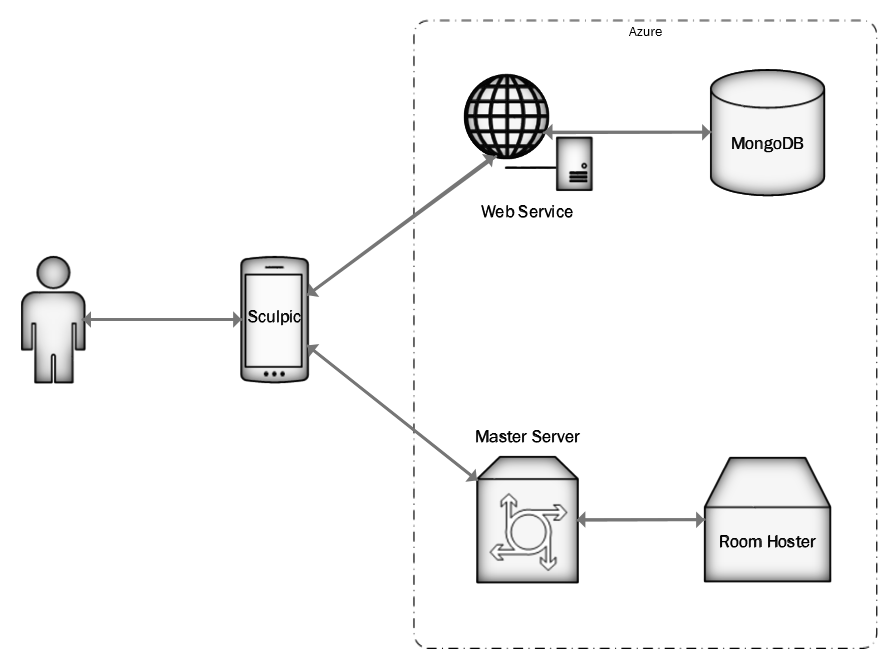
\includegraphics[width=\textwidth]{Architecture}
\caption{Architektura projektu.}
\label{fig:architecture}
\end{figure}

\subsection{Sculpic}
Sculpic jest aplikacją mobilną na platformę Android stworzoną z wykorzystaniem Unity. Z punktu widzenia użytkownika jest to najistotniejsza część projektu, gdyż jedynie z nią użytkownik odbywa interakcję. Łączy się ona z Master Serverem w celu założenia pokoju bądż dołączenia do już istniejącego. Dzięki jego udziałowi pobiera wszelkie informacje o stanie gry z aplikacji hostującej pokój.

\subsection{Azure - maszyna wirtualna}
Na platformie Azure istnieje maszyna wirtualna, na której znajdują się wszystkie elementy związane z serwerową stroną gry.

\subsubsection{Master Server}
Wykorzystujemy aplikację Master Server do obłsugi:
\begin{itemize}
    \item utworzenia pokoju,
    \item dołączenie gracza do pokoju,
    \item przesyłania informacji pomiędzy graczami, m.in:
    \begin{itemize}
        \item zmian zachodzących w obiektach obecnych w grze
        \item wiadomości chatu
        \item punktów
        \item aktualnego rysującego
        \item zgadywanego hasła
    \end{itemize}
\end{itemize}

\subsubsection{Room Hoster}
Room Hoster jest aplikacją, która uruchamia się na maszynie wirtualnej, gdy gracz utworzy pokój. Działa ona dopóki gra w owym pokoju nie zostanie zakończona. Przy pomocy Master Servera komunikuje się z graczami podłączonymi do pokoju, który reprezentuje. Bez Room Hostera niemożliwe jest przeprowadzenie rozgrywki, ponieważ aplikacja ta zarządza głównymi zdarzeniami w grze:
\begin{enumerate}
    \item rozpoczyna grę
    \item utrzymuje kolejkę graczy chcących rysować i wyznacza kolejnego rysującego
    \item rozsyła punkty
    \item kończy grę
    \item uaktualnia ranking
\end{enumerate}

\subsubsection{Web Service}
Web Service jest serwisem napisanym w konwencji architektury REST przy wykorzystaniu technologii WCF. Sculpic komunikuje się z nim poprzez proste zapytania. Serwis ten jest odpowiedzialny za komunikację z bazą danych, czyli:
\begin{enumerate}
    \item przetwarzanie informacji o użytkowniku (tworzenie użytkownika, logowanie, utrzymywanie rankingu)
    \item utrzymywanie listy dostępnych haseł
    \item losowanie hasła dla rysującego gracza
\end{enumerate}

\subsubsection{MongoDB}
MongoDB jest bazą danych, którą wykorzystujemy w naszym projekcie. Przechowuje ona wszystkie informacje o użytkownikach korzystających z aplikacji Sculpic oraz bazę fraz dostępnych w grze. Komunikacja z nia odbywa się przez Web Service.

\section{Dziedzina problemu}
\begin{figure}[htbp]
\centering
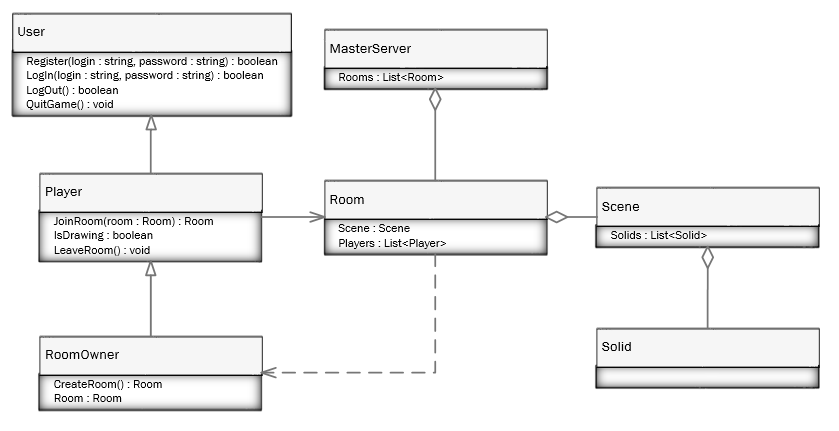
\includegraphics[width=\textwidth]{Domain}
\caption{Dziedzina problemu.}
\label{fig:domain}
\end{figure}

Głównymi składnikami dziedziny są:
\begin{itemize}
    \item użytkownik – osoba korzystająca z aplikacji Sculpic, która może:
    \begin{itemize}
        \item zarejestrować swoje konto w grze,
        \item zalogować się na swoje konto w grze,
        \item występować w poniższych rolach:
        \begin{itemize}
            \item gracz – osoba biorąca udział w grze; może:
            \begin{itemize}
                \item założyć pokój (staje się wtedy również Właścicielem Pokoju),
                \item dołączyć do istniejącego Pokoju,
                \item grać w Pokoju, do którego dołączyła,
                \item wyjść z Pokoju,
                \item wyjść z gry;
            \end{itemize}
            \item właściciel pokoju – gracz, który założył pokój;
        \end{itemize}
    \end{itemize}
    \item Master Server – aplikacja udostępniająca m.in. następujące funkcje:
    \begin{itemize}
        \item zarejestrowanie Pokoju,
        \item dołączenie do Pokoju,
        \item wyjście z Pokoju;
    \end{itemize}
    \item pokój – instancja gry zainicjowana przez Właściciela Pokoju,
    \item scena – przestrzeń w ramach Pokoju na której odbywa się gra,
    \item bryła – obiekt, który Gracz może umieścić na Scenie podczas gry.
\end{itemize}

Rysunek \ref{fig:domain} przedstawia zależności pomiędzy elementami dziedziny.

\section{Struktura bazy danych}
W projekcie wykorzystana jest dokumentowa baza danych, która charakteryzuje się brakiem relacji między poszczególnymi kolekcjami. Dlatego też dane nie są łączone poprzez klucze głównie ani obce, obiekt zawarty w jednym rekordzie stanowi kompletną całość. Dzięki temu pobieranie danych jest dużo wydajniejsze, gdyż bazy dokumentowe nie wspierają tradycyjnych operacji typu JOIN – musiałoby się to odbywać poprzez ręcznie wyszukiwanie rekordów w różnych kolekcjach.

Baza danych projektu składa się z dwóch kolekcji:
\begin{itemize}
    \item Users – zawiera dane logowania użytkowników a także informację o ich rankingu,
    \item Phrases – pełni funkcję spisu haseł losowanych do odgadnięcia w grze, model zawiera również pole wskazujące na ilość wylosowań danej frazy oraz losową liczbę służącą do optymalizacji procesu wyboru hasła.
\end{itemize}

Do wydajnego działania tych kolekcji wystarczą tylko dwa indeksy na pojedynczych polach (Single Field Index). W kolekcji Users jest to pole UserId, natomiast w kolekcji Phrases – RandomNumber.

Warto zaznaczyć, że baza MongoDB pozwala na umieszczanie w kolekcjach obiektów dowolnych typów. Dbanie o spójność i zgodność obiektów w kolekcji leży w kwestii programisty, w naszym projekcie zapewnione jest to przez system repozytoriów.

TODO: Dodać schemat UML klas User, Phrase, jak już będzie ranking

\section{Wzorce projektowe}
Aby zapewnić czystość i przejrzystość kodu oraz logiczną strukturę aplikacji, zdecydowałyśmy się na wykorzystanie kilku znany i sprawdzonych wzorców projektowych, których zastosowanie znacznie wspomogło proces planowania architektury.

\subsection{Singleton}
Wzorzec singleton polega na ograniczeniu ilości istniejących instancji danej klasy do jednej oraz na zapewnieniu dostępu do owego obiektu.

W naszym projekcie wzorzec ten został wykorzystany w klasie Player znajdującej się w grze Sculpic. Z danej instancji gry może korzystać jeden gracz w danym momencie. Jego aktualny stan jest przetrzymywany właśnie w obiekcie klasy Player i musi być dostępny z każdego miejsca w kodzie gry.

\subsection{Repozytorium}
Jest to wzorzec, który ma zastosowanie wszędzie tam, gdzie zachodzi potrzeba odwołania się do danych pobieranych z zewnętrznego źródła takiego jak np. baza danych bądź SharePoint. Polega on na wydzieleniu obsługi operacji związanych z pobieraniem, zapisywaniem i aktualizowaniem każdego modelu do oddzielnej klasy. Repozytorium może zajmować się również mapowaniem modelu bazowego na model biznesowy – jest pośrednikiem między źródłem danych a logiką aplikacji, co ułatwia utrzymanie oraz testowanie funkcjonalności oraz zapewnia przejrzystość architektury. Wzorzec ten ponadto znacznie ogranicza redundancję kodu a także uniezależnia implementację logiki biznesowej aplikacji od użycia konkretnego rodzaju bazy danych.

Najczęstszym zarzutem stawianym temu wzorcowi projektowemu, a także powodem, dla którego często jest on nazywany ”antywzorcem” programowania jest twierdzenie, iż repozytorium łamie zasadę jednej odpowiedzialności klasy, jednak dobrze zaprojektowane repozytorium będzie zawierać jedynie operacje bazodanowe, niezależne od logiki aplikacji, co wydaje się być spójną odpowiedzialnością. 

W naszym projekcie implementacja tego wzorca odbywa się za pomocą następujących komponentów:
\begin{enumerate}
\item Generyczny interfejs IRepository<T> - określa podstawowe operacje bazodanowe możliwe do wykonania na każdym modelu,
\item Generyczna klasa bazowa MongoRepository<T>, implementująca powyższy interfejs – zawiera implementację operacji interfejsu za pomocą sterownika do obsługi bazy Mongo,
\item Interfejsy dla repozytoriów zawierających dodatkowe metody dla każdego typu modelu, dziedziczące po IRepository<T>,
\item	Klasy repozytoriów zawierające implementację dodatkowych metod dla każdego modelu, dziedziczące po klasie MongoRepository oraz implementujące interfejs dla konkretnego modelu
\end{enumerate}

\begin{figure}[htbp]
\centering
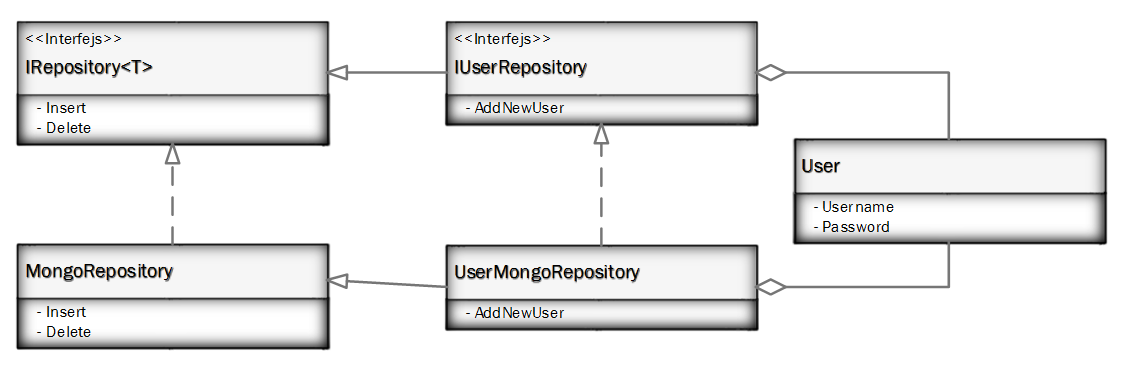
\includegraphics[width=\textwidth]{Repository}
\caption{Przykład zastosowania wzorca Repozytorium.}
\end{figure}

Warto zaznaczyć fakt, iż architektura ta jest bardzo uniwersalna i może służyć do obsługi dowolnej aplikacji korzystającej z bazy danych MongoDB.

\subsection{SOA}
Architektura zorientowana na usługi (Service Oriented Architecture) składa się z dobrze zdefiniowanych serwisów, z których każdy jest niezależnym systemem, akceptującym zapytania oraz zwracającym odpowiedzi za pomocą łatwo dostępnych i jasno określonych interfejsów. Każdy z serwisów może być zmieniany bądź rozbudowywany niezależnie od reszty komponentów wchodzących w skład systemu, co pomaga w łatwym dopasowywaniu się do zmieniających się wymagań biznesowych.

W odróżnieniu od tradycyjnych sposobów tworzenia architektury, które zakładają ścisłe związki oraz współpracę elementów, SOA składa się z luźno powiązanych usług, które wspólnie pozwalają uzyskać pożądane rezultaty. Dodatkowo, implementacja serwisów jest ukryta z punktu widzenia aplikacji klienckiej, zatem wszelakie jej modyfikacje (takie jak optymalizacja bądź dostosowanie do nowych wymagań) nie będą powodowały konieczności wprowadzania zmian w kodzie klienta tak długo, jak nie zmieni się sposób dostępu do usługi.

Kolejną cechą charakterystyczną dla architektury SOA jest również podejście oparte na otwartych i uniwersalnych standardach. Dla przykładu, w naszej implementacji parametry zapytań oraz odpowiedzi przesyłane są w formacie JSON, który może być łatwo obsłużony w niemal każdym współczesnym języku programowania. Zaletą takiego podejścia jest możliwość wykorzystania tych samych usług z poziomu różnych platform, np. aplikacji webowej, aplikacji mobilnej na system Android bądź skryptu używanego przez Unity3D.

Założenia SOA spełnia w naszym systemie serwer bazodanowy. Dzięki temu jest on na tyle uniwersalny, że z jego pomocą możliwa byłaby obsługa grup użytkowników z wielu różnych gier.